\documentclass[11pt,openany,oneside]{book}
\usepackage[a4paper,top=25mm,bottom=23mm,left=25mm,right=22mm,headheight=22pt]{geometry}
\usepackage{fontspec}
\setmainfont{DejaVu Serif}
\setsansfont{DejaVu Sans}
\usepackage{amssymb,xcolor,graphicx,array,booktabs,longtable,tabularx,colortbl,enumitem,tikz,tcolorbox,fancyhdr,titlesec,tocloft,hyperref,eso-pic,microtype}
\usetikzlibrary{arrows.meta,positioning,shapes.geometric,calc}
\definecolor{Navy}{HTML}{17365D}
\definecolor{Teal}{HTML}{007F86}
\definecolor{Pale}{HTML}{EAF6F7}
\definecolor{Gold}{HTML}{E3A72F}
\definecolor{Ink}{HTML}{293746}
\definecolor{LightGold}{HTML}{FFF5DD}
\definecolor{SoftGray}{HTML}{F4F6F9}
\definecolor{Coral}{HTML}{D95D50}
\definecolor{Violet}{HTML}{7656A6}
\definecolor{Sky}{HTML}{DCEEFF}
\definecolor{Rose}{HTML}{FCEBE8}
\hypersetup{colorlinks=true,linkcolor=Teal,urlcolor=Teal,pdftitle={Artificial Intelligence Assistant -- Grade IX},pdfauthor={Vocational Learning Textbook}}
\setlist[itemize]{leftmargin=1.5em,itemsep=1.5pt,topsep=2pt,parsep=0pt}
\setlist[enumerate]{leftmargin=1.7em,itemsep=2pt,topsep=2pt,parsep=0pt}
\setlength{\parindent}{0pt}
\setlength{\parskip}{3pt}
\setlength{\emergencystretch}{3em}
\AddToShipoutPictureBG{\begin{tikzpicture}[remember picture,overlay]\draw[Navy!65,line width=.55pt] ([xshift=11mm,yshift=-11mm]current page.north west) rectangle ([xshift=-11mm,yshift=11mm]current page.south east);\draw[Teal,line width=1.6pt] ([xshift=11mm,yshift=-11mm]current page.north west)--([xshift=37mm,yshift=-11mm]current page.north west);\draw[Coral,line width=1.6pt] ([xshift=-11mm,yshift=11mm]current page.south east)--([xshift=-37mm,yshift=11mm]current page.south east);\fill[Gold] ([xshift=11mm,yshift=-11mm]current page.north west) circle (1.1mm);\fill[Violet] ([xshift=-11mm,yshift=11mm]current page.south east) circle (1.1mm);\end{tikzpicture}}
\pagestyle{fancy}
\fancyhf{}
\fancyhead[L]{\raisebox{-3.5mm}[0pt][0pt]{\small\bfseries\sffamily\color{Teal} ARTIFICIAL INTELLIGENCE ASSISTANT}}
\fancyhead[R]{\raisebox{-3.5mm}[0pt][0pt]{\small\sffamily\color{Navy} GRADE IX TEXTBOOK}}
\fancyfoot[C]{\tikz[baseline=(n.base)]\node[fill=Teal,draw=Gold,line width=.7pt,text=white,circle,minimum size=7mm,inner sep=1pt,font=\small\bfseries] (n) {\thepage};}
\renewcommand{\headrulewidth}{.5pt}
\renewcommand{\headrule}{\hbox to\headwidth{\color{Gold}\leaders\hrule height \headrulewidth\hfill}}
\fancypagestyle{plain}{\fancyhf{}\fancyhead[L]{\raisebox{-3.5mm}[0pt][0pt]{\small\bfseries\sffamily\color{Teal} ARTIFICIAL INTELLIGENCE ASSISTANT}}\fancyhead[R]{\raisebox{-3.5mm}[0pt][0pt]{\small\sffamily\color{Navy} GRADE IX TEXTBOOK}}\fancyfoot[C]{\tikz[baseline=(n.base)]\node[fill=Teal,draw=Gold,line width=.7pt,text=white,circle,minimum size=7mm,inner sep=1pt,font=\small\bfseries] (n) {\thepage};}\renewcommand{\headrulewidth}{.5pt}\renewcommand{\headrule}{\hbox to\headwidth{\color{Gold}\leaders\hrule height \headrulewidth\hfill}}\renewcommand{\footrulewidth}{0pt}}
\titleformat{\chapter}[display]{\normalfont\sffamily\bfseries\color{Navy}}{\filleft\Large\color{Coral}\chaptername\ \thechapter}{.6ex}{\color{Teal}\LARGE\raggedright}[\vspace{.5ex}\color{Gold}\rule{\textwidth}{.8pt}]
\titlespacing*{\chapter}{0pt}{-8mm}{.5ex}
\titlespacing*{\section}{0pt}{1.2ex plus .2ex minus .2ex}{.35ex}
\titlespacing*{\subsection}{0pt}{1ex plus .2ex minus .2ex}{.3ex}
\titleformat{\section}{\Large\sffamily\bfseries\color{Teal}}{\color{Coral}\thesection}{.7em}{}
\titleformat{\subsection}{\large\sffamily\bfseries\color{Violet}}{\thesubsection}{.7em}{}
\newcommand{\exampractice}[1]{\begin{tcolorbox}[colback=LightGold,colframe=Gold,boxrule=.6pt,arc=1.2mm,left=2mm,right=2mm,top=1mm,bottom=1mm]\textbf{Think and answer.} #1\end{tcolorbox}}
\newcommand{\keyterm}[1]{\textbf{\color{Navy}#1}}
\begin{document}
\begin{titlepage}\thispagestyle{empty}
\begin{tikzpicture}[remember picture,overlay]
\fill[Navy] (current page.north west) rectangle ([yshift=-11.4cm]current page.north east);
\fill[Teal] ([yshift=-11.4cm]current page.north west) rectangle ([yshift=-11.68cm]current page.north east);
\fill[Coral] ([yshift=-11.68cm]current page.north west) rectangle ([yshift=-11.82cm]current page.north east);
\draw[Gold,line width=2pt] ([xshift=22mm,yshift=-20mm]current page.north west)--([xshift=-22mm,yshift=-20mm]current page.north east);
\draw[Gold,line width=1pt] ([xshift=22mm,yshift=-103mm]current page.north west)--([xshift=-22mm,yshift=-103mm]current page.north east);
\end{tikzpicture}
\vspace*{20mm}{\color{white}\rmfamily\bfseries\fontsize{38}{44}\selectfont HANDBOOK\par}
\vspace{5mm}{\color{Gold}\rule{.72\textwidth}{1.2pt}\par}
\vspace{7mm}{\color{white}\sffamily\LARGE Artificial Intelligence Assistant\par}
\vspace{3mm}{\color{white}\sffamily\large Grade IX -- Vocational Education\par}
\vfill
\begin{center}{\sffamily\Large\bfseries\color{Teal} AI Concepts \textbullet\ Scratch \textbullet\ Python \textbullet\ Data \textbullet\ Machine Learning\par}\vspace{4mm}{\sffamily\large\color{Ink} A textbook-style learning resource with worked examples, diagrams and review questions\par}\end{center}
\vfill
\begin{center}{\small Based on the supplied Grade IX study material\par}\end{center}
\end{titlepage}
\frontmatter
\tableofcontents
\mainmatter

\chapter{Introduction to Artificial Intelligence}
\section{What is artificial intelligence?}
Artificial Intelligence (AI) is a field of computing concerned with building systems that perform tasks commonly associated with human intelligence. These tasks may include recognising patterns, understanding language, interpreting images, making predictions and selecting actions. An AI system does not have to think exactly like a person; it is designed to perform a particular task using data, rules or learned patterns.

The word \keyterm{artificial} means made by people, while \keyterm{intelligence} includes abilities such as learning, reasoning, understanding information and solving problems. A spam filter, a voice assistant, a translation service and a system that recognises objects in photographs are everyday examples of AI-supported applications.

\begin{center}
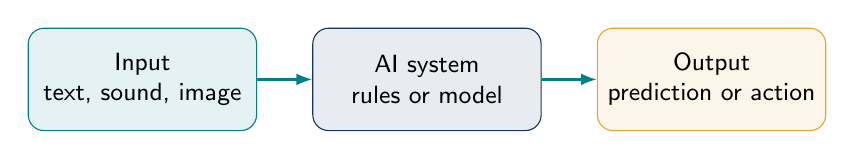
\begin{tikzpicture}[node distance=7mm, every node/.style={font=\small\sffamily,align=center}, box/.style args={#1}{rounded corners=2mm,draw=#1,fill=#1!10,minimum width=29mm,minimum height=13mm}]
\node[box=Teal] (input) {Input\\text, sound, image};
\node[box=Navy,right=of input] (process) {AI system\\rules or model};
\node[box=Gold,right=of process] (output) {Output\\prediction or action};
\draw[-{Latex[length=2mm]},thick,Teal] (input)--(process);
\draw[-{Latex[length=2mm]},thick,Teal] (process)--(output);
\end{tikzpicture}
\end{center}
\textit{Figure 1.1.} A simplified view of how an AI application receives input and produces an output.

\section{Core abilities associated with AI}
\begin{itemize}
\item \keyterm{Learning:} using examples or experience to improve performance on a task.
\item \keyterm{Reasoning:} applying rules or relationships to reach a conclusion.
\item \keyterm{Problem solving:} considering possible steps and selecting a suitable solution.
\item \keyterm{Perception:} interpreting images, sound or other signals from the environment.
\item \keyterm{Language processing:} working with written or spoken human language.
\end{itemize}
Not every AI application uses all these abilities. A simple rule-based system may follow conditions written by a developer, while a machine-learning system may learn useful patterns from examples.

\section{AI in everyday life}
AI-supported features can appear in email spam detection, maps and route suggestions, speech recognition, translation, accessibility tools, shopping recommendations, fraud alerts and image search. In each case, the system uses input data and a designed method to produce a result. The result may be helpful, but it can still be incomplete or incorrect.

\begin{center}
\begin{tikzpicture}[every node/.style={font=\small\sffamily,align=center},aiUseCard/.style={draw=Navy!65,rounded corners=2mm,minimum width=43mm,minimum height=24mm,text width=39mm,inner sep=2mm}]
\node[aiUseCard,fill=Pale] (voice) at (0,0) {\textcolor{Teal}{\Large\textbf{Aa}}\\\textbf{Voice and language}\\Speech recognition and translation};
\node[aiUseCard,fill=LightGold,draw=Gold] (vision) at (5.0,0) {\textcolor{Coral}{\Large\textbf{◎}}\\\textbf{Images and vision}\\Finding objects in photographs};
\node[aiUseCard,fill=Sky,draw=Navy] (suggest) at (10.0,0) {\textcolor{Violet}{\Large\textbf{↗}}\\\textbf{Predictions}\\Route suggestions and spam alerts};
\end{tikzpicture}
\end{center}
\textit{Figure 1.4.} Examples of everyday tasks where AI-supported features may be used.

\section{Why learn AI at school?}
Learning AI helps students understand digital services they already use and develop the vocabulary needed to discuss them. It also builds habits of logical thinking, careful observation, data interpretation and responsible technology use. Students can begin with visual programming and gradually move towards text-based programming and data projects.

\section{Types of Artificial Intelligence}
AI can be grouped in more than one way. One common classroom explanation groups it by the range of tasks it could perform. Another describes how a system behaves or uses information. These are useful learning frameworks, not proof that every category already exists as a real product.

\subsection{Types based on capability}
\begin{itemize}
\item \keyterm{Narrow AI (ANI):} designed for a specific task or a limited set of related tasks. Examples include speech recognition, spam filtering and route suggestions. Most AI applications used today fall into this category.
\item \keyterm{Artificial General Intelligence (AGI):} a proposed system that could learn and perform a broad range of intellectual tasks at a flexible, human-like level. It has not been established as a generally available system.
\item \keyterm{Artificial Superintelligence (ASI):} a hypothetical concept describing AI that would exceed human abilities across many important areas. It is an idea discussed in research and public debate, not an established current technology.
\end{itemize}

\begin{center}
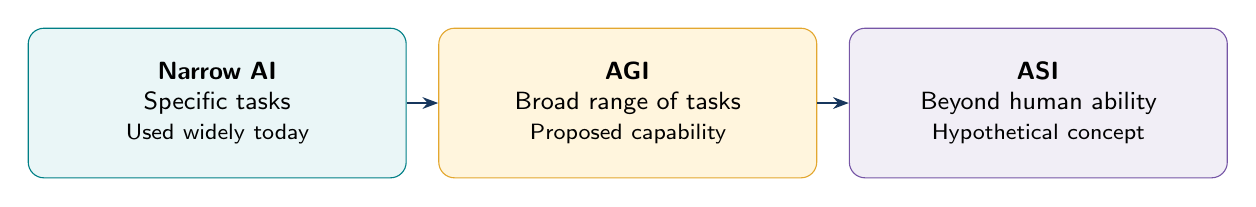
\begin{tikzpicture}[node distance=4mm,every node/.style={font=\small\sffamily,align=center},aiCapabilityBox/.style={draw=Teal,fill=Pale,rounded corners=2mm,text width=42mm,minimum height=19mm,inner sep=3mm},aiDiagramArrow/.style={-{Stealth[length=2mm]},draw=Navy,line width=.7pt}]
\node[aiCapabilityBox] (ani) {\textbf{Narrow AI}\\Specific tasks\\\footnotesize Used widely today};
\node[aiCapabilityBox,right=of ani,draw=Gold,fill=LightGold] (agi) {\textbf{AGI}\\Broad range of tasks\\\footnotesize Proposed capability};
\node[aiCapabilityBox,right=of agi,draw=Violet,fill=Violet!10] (asi) {\textbf{ASI}\\Beyond human ability\\\footnotesize Hypothetical concept};
\draw[aiDiagramArrow] (ani)--(agi);
\draw[aiDiagramArrow] (agi)--(asi);
\end{tikzpicture}
\end{center}
\textit{Figure 1.2.} Capability categories, from task-specific AI to broader hypothetical capabilities. The arrows show a conceptual progression, not a guaranteed development path.

\subsection{Types based on how a system works}
\begin{itemize}
\item \keyterm{Reactive machines:} respond to the current input using a defined method, without storing experiences to improve future decisions. They are a simple conceptual category.
\item \keyterm{Limited-memory AI:} uses recent data or information from past observations to support a task. Many modern AI applications use some form of stored context or historical data, although the details differ.
\item \keyterm{Theory-of-mind AI:} a proposed type that would interpret other people's beliefs, intentions or emotions in a deeper, context-aware way. Current systems may recognise cues but can misunderstand what people actually think or feel.
\item \keyterm{Self-aware AI:} a hypothetical system with genuine self-awareness. There is no established evidence that today's AI systems are self-aware.
\end{itemize}

\begin{center}
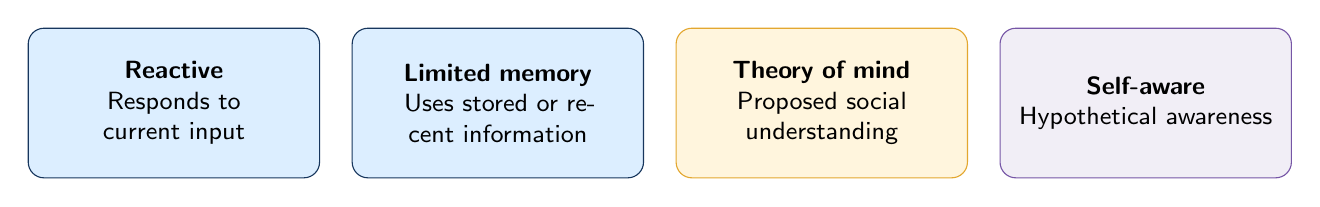
\begin{tikzpicture}[node distance=4mm,every node/.style={font=\small\sffamily,align=center},aiFunctionBox/.style={draw=Navy,fill=Sky,rounded corners=2mm,text width=33mm,minimum height=19mm,inner sep=2mm}]
\node[aiFunctionBox] (react) {\textbf{Reactive}\\Responds to current input};
\node[aiFunctionBox,right=of react] (memory) {\textbf{Limited memory}\\Uses stored or recent information};
\node[aiFunctionBox,right=of memory,draw=Gold,fill=LightGold] (mind) {\textbf{Theory of mind}\\Proposed social understanding};
\node[aiFunctionBox,right=of mind,draw=Violet,fill=Violet!10] (self) {\textbf{Self-aware}\\Hypothetical awareness};
\end{tikzpicture}
\end{center}
\textit{Figure 1.3.} A simplified comparison of functional categories often used to introduce AI. The last two categories remain theoretical.


\section{Responsible use of AI}
AI outputs should be checked, particularly when a decision affects a person's safety, education, finances or opportunities. Avoid entering private information into tools unless their data practices are understood and authorised. Consider fairness, privacy, transparency, accessibility and the possibility that a model may make mistakes. Human judgement remains important.

\section{Chapter questions}
\begin{enumerate}
\item Define artificial intelligence in your own words.
\item Name four abilities associated with AI and give one example for each.
\item Explain two uses of AI in everyday life.
\item Name the three capability-based types of AI and give one-line descriptions.
\item Which functional categories of AI are considered hypothetical, and why?
\item What is the difference between narrow AI and the idea of AGI?
\item Why should AI-generated results be checked before they are used?
\end{enumerate}

\chapter{Programming Basics and Algorithms}
\section{What is programming?}
Programming is the process of writing instructions that a computer can execute. A program translates a solution into steps that are precise enough for a computer to follow. Programming is used to create websites, games, mobile applications, data tools and AI systems.

\section{Algorithms and logical steps}
An \keyterm{algorithm} is a finite, ordered set of steps for solving a problem. Before writing code, it is useful to state the problem, identify the required input, decide the processing steps and describe the expected output. A clear algorithm is easier to test and improve than a collection of unplanned instructions.

\begin{center}
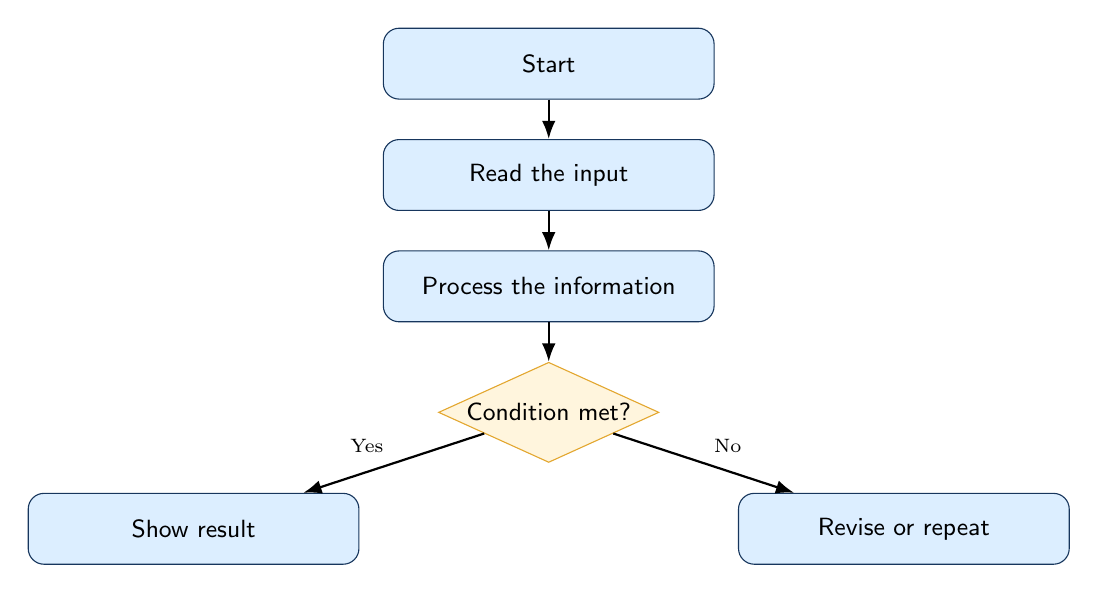
\begin{tikzpicture}[node distance=5mm, every node/.style={font=\small\sffamily,align=center}, process/.style={draw=Navy,fill=Sky,rounded corners=2mm,minimum width=42mm,minimum height=9mm}, decision/.style={draw=Gold,fill=LightGold,diamond,aspect=2.2,inner sep=1pt}]
\node[process] (start) {Start};
\node[process,below=of start] (input) {Read the input};
\node[process,below=of input] (work) {Process the information};
\node[decision,below=of work] (check) {Condition met?};
\node[process,below left=7mm and 17mm of check] (yes) {Show result};
\node[process,below right=7mm and 17mm of check] (no) {Revise or repeat};
\draw[-{Latex},thick] (start)--(input);
\draw[-{Latex},thick] (input)--(work);
\draw[-{Latex},thick] (work)--(check);
\draw[-{Latex},thick] (check)--node[above left,font=\scriptsize]{Yes}(yes);
\draw[-{Latex},thick] (check)--node[above right,font=\scriptsize]{No}(no);
\end{tikzpicture}
\end{center}
\textit{Figure 2.1.} A flowchart shows the order of steps and decisions in an algorithm.

\section{Sequence, selection and repetition}
\keyterm{Sequence} means instructions run in order. \keyterm{Selection} chooses between alternatives using a condition, such as whether a value is greater than zero. \keyterm{Iteration} repeats a set of instructions until a condition is met or a fixed number of repetitions has completed. These three structures are common in many programming languages.

\section{Variables, input and output}
A variable is a named place for a value used by a program. Input is information supplied to the program; output is the result presented to the user or another system. For example, a program may read two numbers, add them and display the sum. Meaningful variable names and consistent indentation make code easier to read.

\section{Testing and debugging}
Testing checks whether a program behaves as expected. Try ordinary values, boundary values and unexpected inputs. Debugging is the process of locating and correcting the cause of a problem. A useful approach is to reproduce the error, inspect the relevant steps, change one thing at a time and test again.

\section{Chapter questions}
\begin{enumerate}
\item What is an algorithm? Why should it be planned before coding?
\item Explain sequence, selection and iteration with examples.
\item What is the purpose of a variable?
\item Distinguish testing from debugging.
\item Draw a flowchart for deciding whether a number is positive or not positive.
\end{enumerate}

\chapter{Coding with Scratch}
\section{Introducing block-based programming}
Scratch is a visual programming environment in which programs are assembled from connected blocks. It helps learners explore computational thinking without needing to memorise punctuation and syntax at the beginning. A project can include sprites, backdrops, sounds, events, motion, looks, sensing and control blocks.

\section{The Scratch workspace}
The Stage displays the project while sprites are the characters or objects that perform actions. The Blocks Palette contains programming blocks, the Code Area is where blocks are connected, and the Sprite List helps select and manage project objects. A backdrop changes the Stage background.

\begin{center}
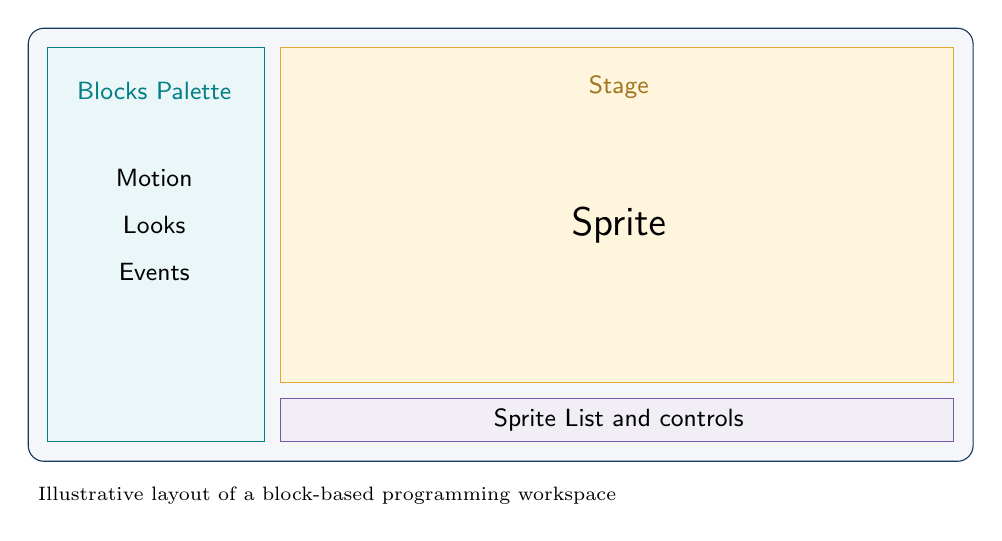
\begin{tikzpicture}[every node/.style={font=\small\sffamily,align=center}]
\draw[draw=Navy,rounded corners=2mm,fill=SoftGray] (0,0) rectangle (12,5.5);
\draw[draw=Teal,fill=Pale] (.25,.25) rectangle (3.0,5.25);
\draw[draw=Gold,fill=LightGold] (3.2,1.0) rectangle (11.75,5.25);
\draw[draw=Violet,fill=Violet!10] (3.2,.25) rectangle (11.75,.8);
\node[text=Teal] at (1.6,4.7) {Blocks Palette};
\node at (1.6,3.6) {Motion};
\node at (1.6,3.0) {Looks};
\node at (1.6,2.4) {Events};
\node[text=Gold!70!black] at (7.5,4.75) {Stage};
\node at (7.5,3.0) {\Large Sprite};
\node at (7.5,.52) {Sprite List and controls};
\node[anchor=north west,font=\scriptsize] at (0,-.2) {Illustrative layout of a block-based programming workspace};
\end{tikzpicture}
\end{center}

\section{Events and motion}
An event block starts a script when something happens, such as clicking the green flag or pressing a key. Motion blocks move a sprite, turn it or change its position. Looks blocks change appearance, costumes or speech bubbles. Combining event and motion blocks can create a simple interactive animation.

\section{Control and sensing}
Control blocks repeat actions, wait for a period or run instructions only when a condition is true. Sensing blocks detect events or information, such as whether a sprite touches another object. Operators perform comparisons and calculations. Variables can store a score, a timer or the number of attempts.

\section{Planning a simple project}
For a simple catching game, define the goal first: the player moves a sprite to catch a falling object. Decide which keys control movement, how a catch is detected, how the score changes and when the game ends. Build one feature at a time and test it before adding sound or extra levels. Keep the rules clear so another learner can understand the game.

\begin{center}
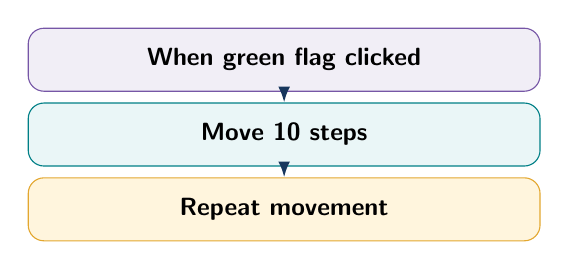
\begin{tikzpicture}[every node/.style={font=\small\sffamily,align=left},scratchEvent/.style={draw=Violet,fill=Violet!10,rounded corners=2mm,minimum width=65mm,minimum height=8mm,inner sep=2mm},scratchMotion/.style={draw=Teal,fill=Pale,rounded corners=2mm,minimum width=65mm,minimum height=8mm,inner sep=2mm},scratchControl/.style={draw=Gold,fill=LightGold,rounded corners=2mm,minimum width=65mm,minimum height=8mm,inner sep=2mm}]
\node[scratchEvent] (event) at (0,0) {\textbf{When green flag clicked}};
\node[scratchMotion] (move) at (0,-.95) {\textbf{Move 10 steps}};
\node[scratchControl] (repeat) at (0,-1.9) {\textbf{Repeat movement}};
\draw[-{Latex[length=2mm]},thick,Navy] (event)--(move);
\draw[-{Latex[length=2mm]},thick,Navy] (move)--(repeat);
\end{tikzpicture}
\end{center}
\textit{Figure 3.1.} A simplified Scratch script: an event starts the action, then motion instructions run. Real Scratch blocks have their own shapes and colours.

\section{Common errors}
Disconnected blocks do not run as part of the intended script. A script may begin with the wrong event, repeat forever or check a condition before the sprite reaches the target. Test with slow movement first, then adjust speed and timing. Give sprites and variables meaningful names.

\section{Chapter questions}
\begin{enumerate}
\item Name four main areas of the Scratch workspace.
\item What is the role of an event block?
\item How are control blocks different from motion blocks?
\item Describe the steps needed to plan a simple catching game.
\item Give two ways to find errors in a Scratch project.
\end{enumerate}

\chapter{Introduction to Python}
\section{What is Python?}
Python is a high-level programming language known for readable syntax. It is used for automation, web development, data analysis, scientific work and many AI projects. Python programs are written as text and executed by a Python interpreter. The exact interface depends on the installed environment.

\section{A first program}
The statement below displays a message:
\begin{tcolorbox}[colback=SoftGray,colframe=Navy,boxrule=.5pt,arc=1mm]
\texttt{print("Hello, AI!")}
\end{tcolorbox}
The function \texttt{print()} sends information to the output. Text placed inside quotation marks is a string. Parentheses group the value passed to the function.

\begin{center}
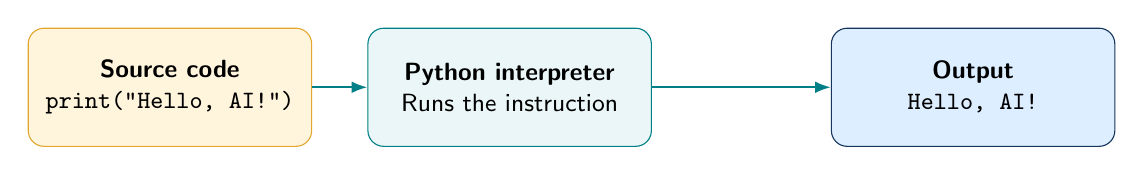
\begin{tikzpicture}[node distance=7mm,every node/.style={font=\small\sffamily,align=center},pyStage/.style={draw=Navy,rounded corners=2mm,minimum width=36mm,minimum height=15mm,inner sep=2mm}]
\node[pyStage,fill=LightGold,draw=Gold] (source) {\textbf{Source code}\\\texttt{print("Hello, AI!")}};
\node[pyStage,fill=Pale,draw=Teal,right=of source] (run) {\textbf{Python interpreter}\\Runs the instruction};
\node[pyStage,fill=Sky] (result) at (10.2,0) {\textbf{Output}\\\texttt{Hello, AI!}};
\draw[-{Latex[length=2mm]},thick,Teal] (source)--(run);
\draw[-{Latex[length=2mm]},thick,Teal] (run)--(result);
\end{tikzpicture}
\end{center}
\textit{Figure 4.1.} A short Python statement is interpreted and produces visible output.

\section{Comments and indentation}
A comment begins with the \texttt{\#} symbol and is ignored when the program runs. Comments explain why a step is needed. Indentation marks the body of many Python structures, such as conditional statements and loops. Inconsistent indentation can cause an error, so use a consistent style.

\section{Reading input and displaying output}
\begin{tcolorbox}[colback=SoftGray,colframe=Navy,boxrule=.5pt,arc=1mm]
\texttt{name = input("Enter your name: ")}\\
\texttt{print("Welcome", name)}
\end{tcolorbox}
The \texttt{input()} function reads text from the user. A value read with \texttt{input()} is a string by default. If a program needs a number, it must convert the text carefully, for example with \texttt{int()} for a whole number.

\section{Errors in Python}
A syntax error means the code does not follow the language rules. A runtime error occurs while the program is executing. A logic error means the program runs but produces an incorrect result. Read the error message, check the line it identifies and test a small example to isolate the problem.

\section{Chapter questions}
\begin{enumerate}
\item What is Python used for?
\item Write a Python statement that prints your school name.
\item What is a comment, and how is it written in Python?
\item Why is indentation important?
\item Distinguish syntax, runtime and logic errors.
\end{enumerate}

\chapter{Data Types and Operators}
\section{Why data types matter}
A data type describes the kind of value a variable holds. Choosing a suitable type helps a program perform the intended operation and prevents avoidable errors. Common introductory Python types include integers, floating-point numbers, strings and Boolean values.

\begin{center}
\begin{tabularx}{\textwidth}{>{\bfseries}p{.2\textwidth} X X}
\toprule
Type & Meaning & Example\\
\midrule
\texttt{int} & Whole number & \texttt{students = 32}\\
\texttt{float} & Number with a decimal part & \texttt{temperature = 28.5}\\
\texttt{str} & Text & \texttt{city = "Bhopal"}\\
\texttt{bool} & True or false value & \texttt{is\_ready = True}\\
\bottomrule
\end{tabularx}
\end{center}

\section{Arithmetic operators}
Python supports addition (\texttt{+}), subtraction (\texttt{-}), multiplication (\texttt{*}), division (\texttt{/}), floor division (\texttt{//}), remainder (\texttt{\%}) and exponentiation (\texttt{**}). Use parentheses to make the intended order of operations clear. Division by zero is invalid and should be handled when user input is involved.

\section{Comparison and logical operators}
Comparison operators such as \texttt{==}, \texttt{!=}, \texttt{>}, \texttt{<}, \texttt{>=} and \texttt{<=} produce Boolean results. Logical operators \texttt{and}, \texttt{or} and \texttt{not} combine or reverse conditions. They are often used in decisions and loops.

\section{Small worked example}
\begin{tcolorbox}[colback=SoftGray,colframe=Navy,boxrule=.5pt,arc=1mm]
\texttt{marks = 76}\\
\texttt{if marks >= 35:}\\
\texttt{\ \ \ \ print("Pass")}\\
\texttt{else:}\\
\texttt{\ \ \ \ print("Try again")}
\end{tcolorbox}
The condition is evaluated as true or false. The program prints one message depending on the result. In a complete application, the value should be read and validated rather than fixed in the source code.

\section{Chapter questions}
\begin{enumerate}
\item List four common Python data types.
\item Explain the difference between \texttt{=} and \texttt{==}.
\item What result does the remainder operator produce?
\item Give an example of a logical condition using \texttt{and}.
\item Write a short program that checks whether a number is greater than zero.
\end{enumerate}

\chapter{Basics of Data Literacy}
\section{Understanding data}
Data are recorded observations, values or descriptions. They may be numerical, textual, categorical, visual or audio-based. Information is produced when data are organised and interpreted in a context. Data literacy is the ability to read, question, analyse and communicate information from data responsibly.

\section{Sources and types of data}
Data may come from surveys, forms, sensors, observations, transactions or existing datasets. Primary data are collected directly for a purpose; secondary data were collected earlier by another person or organisation. Quantitative data describe counts or measurements. Qualitative data describe qualities or categories. Before using a dataset, identify its source, purpose, units, time period and any limitations.

\section{A basic data workflow}
\begin{center}
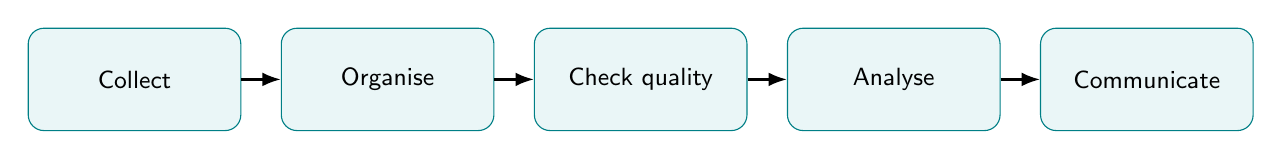
\begin{tikzpicture}[node distance=5mm,every node/.style={font=\small\sffamily,align=center},flowstep/.style={draw=Teal,fill=Pale,rounded corners=2mm,minimum width=27mm,minimum height=13mm}]
\node[flowstep] (collect) {Collect};
\node[flowstep,right=of collect] (organise) {Organise};
\node[flowstep,right=of organise] (check) {Check quality};
\node[flowstep,right=of check] (analyse) {Analyse};
\node[flowstep,right=of analyse] (share) {Communicate};
\draw[-{Latex},thick] (collect)--(organise);
\draw[-{Latex},thick] (organise)--(check);
\draw[-{Latex},thick] (check)--(analyse);
\draw[-{Latex},thick] (analyse)--(share);
\end{tikzpicture}
\end{center}

\section{Reading a dataset}
A dataset arranged in rows and columns often uses each row for one record and each column for one variable. A column heading should clearly describe the values below it. Check whether units are consistent, whether values are missing and whether the same record appears more than once. A surprising value is a reason to investigate, not automatically a reason to delete it.

\section{Privacy and fairness}
Collect only data needed for a legitimate purpose. Do not publish personal details without appropriate permission. A dataset may under-represent a group or reflect past unfair decisions. Ask who is included, who is missing and how conclusions may affect different people. Good data practice includes secure storage, careful access and honest communication of uncertainty.

\section{Chapter questions}
\begin{enumerate}
\item Define data literacy.
\item Distinguish primary and secondary data.
\item Explain quantitative and qualitative data with examples.
\item Name four checks that can improve data quality.
\item Why should a dataset's source and limitations be documented?
\end{enumerate}

\chapter{Data Pre-processing}
\section{Why data need preparation}
Collected data are often inconsistent or incomplete. Data pre-processing is the set of steps used to inspect and prepare data before analysis or machine learning. Poor-quality input can lead to misleading summaries and unreliable model predictions. Preparation should be appropriate to the question being studied.

\section{Common data-quality issues}
Missing values occur when a field has not been recorded. Duplicates represent repeated records. Inconsistent formats may use different spellings, date patterns or units. Invalid values fall outside the rules for a field. Outliers are unusually high or low values; they may be genuine observations or errors and require investigation.

\section{A careful cleaning process}
\begin{enumerate}
\item Keep an unchanged copy of the original dataset.
\item Inspect column names, data types, units and sample records.
\item Identify missing values, duplicates and inconsistent formats.
\item Decide how each issue should be handled and record the reason.
\item Validate the cleaned data and compare it with the original.
\end{enumerate}
Do not automatically replace every missing value with zero: zero may have a real meaning. Depending on the task, a missing value may be left unknown, filled using a justified method or excluded with a clear explanation.

\begin{center}
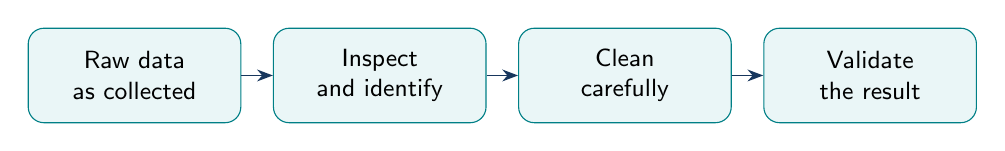
\begin{tikzpicture}[node distance=4mm,every node/.style={font=\small\sffamily,align=center},stepbox/.style={draw=Teal,fill=Pale,rounded corners=2mm,minimum width=27mm,minimum height=12mm},aiDiagramArrow/.style={-{Stealth[length=2mm]},draw=Navy,line width=.7pt}]
\node[stepbox] (raw) {Raw data\\as collected};
\node[stepbox,right=of raw] (inspect) {Inspect\\and identify};
\node[stepbox,right=of inspect] (clean) {Clean\\carefully};
\node[stepbox,right=of clean] (check) {Validate\\the result};
\draw[aiDiagramArrow] (raw)--(inspect);
\draw[aiDiagramArrow] (inspect)--(clean);
\draw[aiDiagramArrow] (clean)--(check);
\end{tikzpicture}
\end{center}
\textit{Figure 7.1.} A simple data-cleaning workflow. Keep the original data and record important changes.

\section{Preparing data for machine learning}
For supervised learning, input features and the target label must be identified. Categorical data may need encoding and numerical features may need scaling for some algorithms. Split data into training and test sets before using test results to make decisions. Any transformation that learns from data should be fitted using the training data only, to reduce information leakage.

\section{Chapter questions}
\begin{enumerate}
\item What is data pre-processing?
\item Give three examples of data-quality problems.
\item Why should the original dataset be preserved?
\item Why is replacing every missing value with zero unsafe?
\item Explain the purpose of a training and test split.
\end{enumerate}

\chapter{Mathematics for AI: Data Analysis}
\section{Why mathematics is useful}
Mathematics helps describe data, compare values and reason about patterns. Basic arithmetic, fractions, percentages, averages, ratios and simple graphs are useful when interpreting data. Mathematical summaries do not replace context: the same number can mean different things depending on how data were collected.

\section{Counts, totals and averages}
The total is the sum of values. The mean is the total divided by the number of values. The median is the middle value after sorting, and the mode is the most frequent value. The mean can be affected by extreme values, while the median is often more resistant to them.

\begin{center}
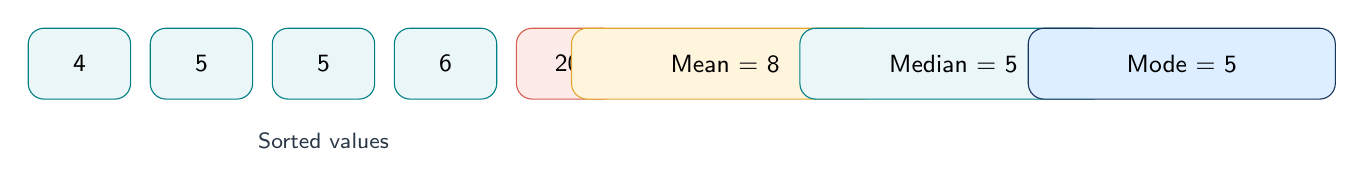
\begin{tikzpicture}[every node/.style={font=\small\sffamily,align=center}]
\node[draw=Teal,fill=Pale,rounded corners=2mm,minimum width=13mm,minimum height=9mm] (v1) at (0,0) {4};
\node[draw=Teal,fill=Pale,rounded corners=2mm,minimum width=13mm,minimum height=9mm] (v2) at (1.55,0) {5};
\node[draw=Teal,fill=Pale,rounded corners=2mm,minimum width=13mm,minimum height=9mm] (v3) at (3.1,0) {5};
\node[draw=Teal,fill=Pale,rounded corners=2mm,minimum width=13mm,minimum height=9mm] (v4) at (4.65,0) {6};
\node[draw=Coral,fill=Rose,rounded corners=2mm,minimum width=13mm,minimum height=9mm] (v5) at (6.2,0) {20};
\node[font=\footnotesize\sffamily,text=Ink,below=3mm of v3] {Sorted values};
\node[draw=Gold,fill=LightGold,rounded corners=2mm,minimum width=39mm,minimum height=9mm] at (8.2,0) {Mean = 8};
\node[draw=Teal,fill=Pale,rounded corners=2mm,minimum width=39mm,minimum height=9mm] at (11.1,0) {Median = 5};
\node[draw=Navy,fill=Sky,rounded corners=2mm,minimum width=39mm,minimum height=9mm] at (14,0) {Mode = 5};
\end{tikzpicture}
\end{center}
\textit{Figure 8.2.} A compact visual summary of one dataset. The unusually large value 20 pulls the mean above the median and mode.

\section{Percentages and ratios}
A percentage expresses a part out of one hundred. The percentage of a group meeting a condition is calculated as the number meeting the condition divided by the total number, multiplied by 100. A ratio compares quantities. Always state the denominator and the population being compared so that a percentage is not misinterpreted.

\section{Correlation and caution}
Two variables may change together, but this does not prove that one causes the other. A third factor may influence both, or the pattern may be coincidental. When interpreting data, distinguish observation from explanation and avoid claims that go beyond the evidence.

\section{Chapter questions}
\begin{enumerate}
\item Calculate the mean of 6, 8, 10 and 12.
\item Find the median of 3, 7, 9, 12 and 18.
\item How is a percentage calculated?
\item Why can the median be more useful than the mean for data with extreme values?
\item Explain why correlation does not by itself prove causation.
\end{enumerate}

\chapter{Data Visualisation}
\section{Choosing a chart}
Data visualisation presents information in a visual form so that patterns and comparisons can be noticed. A bar chart compares categories; a line chart shows change over an ordered sequence such as time; a pie chart may show parts of a whole when there are only a few categories; and a scatter plot shows the relationship between two numerical variables.

\begin{center}
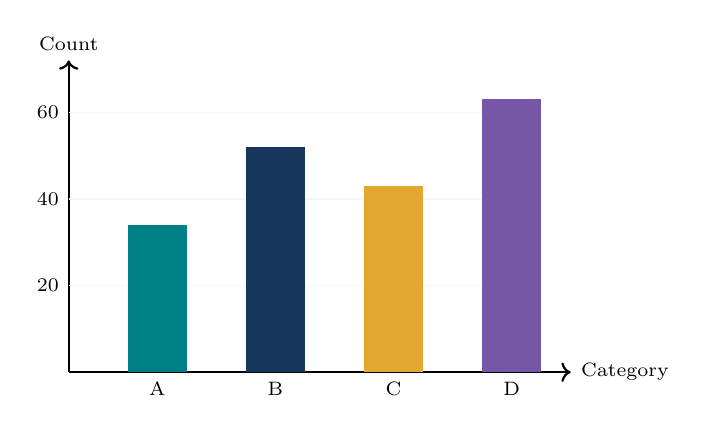
\begin{tikzpicture}[x=0.75cm,y=0.055cm]
\draw[->,thick] (0,0)--(8.5,0) node[right,font=\scriptsize]{Category};
\draw[->,thick] (0,0)--(0,72) node[above,font=\scriptsize]{Count};
\foreach \y in {20,40,60}{\draw[SoftGray] (0,\y)--(8,\y); \node[left,font=\scriptsize] at (0,\y){\y};}
\fill[Teal] (1,0) rectangle (2,34);
\fill[Navy] (3,0) rectangle (4,52);
\fill[Gold] (5,0) rectangle (6,43);
\fill[Violet] (7,0) rectangle (8,63);
\node[below,font=\scriptsize] at (1.5,0){A};
\node[below,font=\scriptsize] at (3.5,0){B};
\node[below,font=\scriptsize] at (5.5,0){C};
\node[below,font=\scriptsize] at (7.5,0){D};
\end{tikzpicture}
\end{center}
\textit{Figure 8.1.} An illustrative bar chart. Values are examples, not measurements from the source material.

\section{Make a chart understandable}
Every chart should have a descriptive title, labelled axes where needed, clear units and a scale that does not mislead. Use a legend only when multiple series need identification. Avoid decorative effects that make comparisons difficult. If values are estimates or incomplete, explain that limitation.

\section{Interpreting visual information}
Read the title and labels first. Check the scale before comparing bar heights or slopes. Look for the largest and smallest values, changes over time and unusual points. Do not infer a cause from a chart alone. A chart should support a conclusion that can also be explained in words.

\section{Chapter questions}
\begin{enumerate}
\item Which chart is suitable for comparing categories?
\item When is a line chart useful?
\item Name four features of a clear chart.
\item How can a graph mislead a reader?
\item Why should the source and units of plotted data be stated?
\end{enumerate}

\chapter{Introduction to Machine Learning}
\section{What is machine learning?}
Machine Learning (ML) is a part of AI in which a system uses data to learn patterns that help it make predictions or decisions. Instead of writing a separate rule for every possible case, a developer chooses a method, supplies suitable examples and evaluates the resulting model. ML performance depends on the data, the task and the way the model is tested.

\section{A typical machine-learning workflow}
\begin{center}
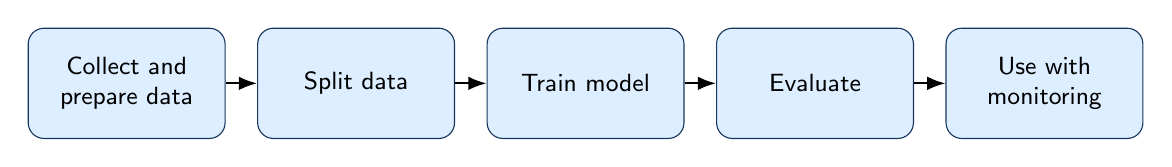
\begin{tikzpicture}[node distance=4mm,every node/.style={font=\small\sffamily,align=center},flowstep/.style={draw=Navy,fill=Sky,rounded corners=2mm,minimum width=25mm,minimum height=14mm}]
\node[flowstep] (data) {Collect and\\prepare data};
\node[flowstep,right=of data] (split) {Split data};
\node[flowstep,right=of split] (train) {Train model};
\node[flowstep,right=of train] (test) {Evaluate};
\node[flowstep,right=of test] (use) {Use with\\monitoring};
\draw[-{Latex},thick] (data)--(split);
\draw[-{Latex},thick] (split)--(train);
\draw[-{Latex},thick] (train)--(test);
\draw[-{Latex},thick] (test)--(use);
\end{tikzpicture}
\end{center}

\section{Features, labels and models}
A \keyterm{feature} is an input used by a model, such as the size or colour of an object. A \keyterm{label} is the answer associated with an example in a labelled dataset. A \keyterm{model} is the learned pattern or relationship used to produce an output. Training adjusts the model based on examples; evaluation checks how well it works on data not used for training.

\section{Overfitting and evaluation}
A model may memorise details of training examples instead of learning patterns that generalise. This is called overfitting. Testing with separate data gives a more realistic indication of performance on new cases. Accuracy can be useful, but it may hide important errors when classes are imbalanced. Consider the consequences of false positives and false negatives for the task.

\section{Limits of machine learning}
ML systems can reflect gaps and bias in their training data. A model may perform well in one setting and poorly in another. Predictions are not guarantees. Systems used in real settings need monitoring, privacy safeguards, appropriate human oversight and a way to report problems.

\section{Chapter questions}
\begin{enumerate}
\item Define machine learning and explain its relationship to AI.
\item What are features, labels and models?
\item Why should evaluation data be kept separate from training data?
\item What is overfitting?
\item Give two limitations or risks of ML systems.
\end{enumerate}

\chapter{Types of Machine Learning}
\section{Supervised learning}
Supervised learning uses examples that include inputs and known target labels. A classification model predicts a category, such as whether an email is likely to be spam. A regression model predicts a numerical value, such as an estimated measurement. The quality of the labels and the relevance of the examples affect the result.

\section{Unsupervised learning}
Unsupervised learning works with data that do not have target labels supplied for each example. A method may group similar records or identify structure in the data. Clustering can help explore patterns, but the groups need interpretation and are not automatically meaningful categories.

\section{Reinforcement learning}
In reinforcement learning, an agent takes actions in an environment and receives feedback in the form of rewards or penalties. The agent learns a strategy that aims to improve long-term reward. This approach is used in some control, robotics and game-playing tasks. A reward design that does not match the real goal can lead to undesirable behaviour.

\begin{center}
\begin{tabularx}{\textwidth}{>{\bfseries}p{.22\textwidth} X X}
\toprule
Learning type & Training information & Example task\\
\midrule
Supervised & Inputs with known labels or target values & Classify messages as spam or not spam\\
Unsupervised & Inputs without target labels & Explore groups of similar records\\
Reinforcement & Actions, environment feedback and rewards & Learn a strategy in a simulated game\\
\bottomrule
\end{tabularx}
\end{center}

\section{Deep learning}
Deep learning uses neural networks with multiple processing layers to learn representations from data. It can be effective for images, audio, language and other complex inputs, but it often needs substantial data and computing resources. Deep learning is one family of methods within machine learning, not a synonym for all AI.

\begin{center}
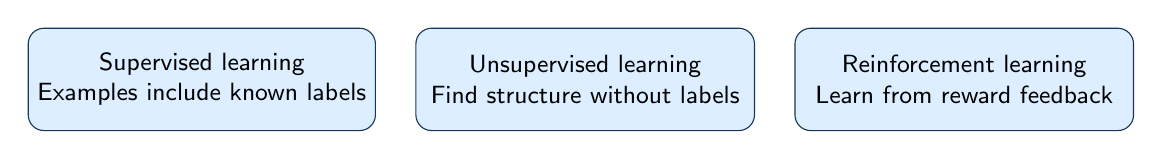
\begin{tikzpicture}[node distance=5mm,every node/.style={font=\small\sffamily,align=center},mlbox/.style={draw=Navy,fill=Sky,rounded corners=2mm,minimum width=43mm,minimum height=13mm}]
\node[mlbox] (sup) {Supervised learning\\Examples include known labels};
\node[mlbox,right=of sup] (unsup) {Unsupervised learning\\Find structure without labels};
\node[mlbox,right=of unsup] (rein) {Reinforcement learning\\Learn from reward feedback};
\end{tikzpicture}
\end{center}
\textit{Figure 10.1.} Three common learning approaches differ in the kind of feedback or information available.

\section{Selecting an approach}
Start with the problem and the available data. If examples have correct labels, supervised learning may be suitable. If the aim is to explore structure without labels, an unsupervised method may help. If actions influence an environment and feedback is available, reinforcement learning may be relevant. The choice should be tested rather than assumed.

\section{Chapter questions}
\begin{enumerate}
\item Explain supervised learning with an example.
\item How does unsupervised learning differ from supervised learning?
\item What role does a reward play in reinforcement learning?
\item What is deep learning?
\item Match a suitable learning type to a spam filter, customer grouping and a game-playing agent.
\end{enumerate}

\end{document}
